\documentclass[conference]{IEEEtran}
\usepackage{amsmath,amssymb,amsfonts}
\usepackage{booktabs}
\usepackage{graphicx}
\usepackage{textcomp}
\usepackage{xcolor}
\usepackage[hidelinks]{hyperref}
\usepackage{multirow}
\usepackage{array}
\graphicspath{{figures/}}

\title{From Fine-Tuning to Edge Deployment: Quantizing\\
Vision--Language--Action Policies for Real Robot Hardware}

\author{
\IEEEauthorblockN{Justin Williams, Kishor Datta Gupta, Roy George, Mrinmoy Sarkar}
\IEEEauthorblockA{Clark Atlanta University, Atlanta, GA 30314\\
Supported by the Air Force Research Laboratory (AFRL) and the Griffiss Institute\\
\texttt{justinwilliamstech693@gmail.com}}
}

\begin{document}
\maketitle

\begin{abstract}
Vision--Language--Action (VLA) policies built on 7B-parameter language backbones deliver
state-of-the-art closed-loop task success but demand 15+ GB of memory and server-class
power, precluding deployment on the embedded compute a mobile robot can carry.
We present an end-to-end study: \textbf{(i) fine-tuning} an OpenVLA-OFT policy on LIBERO
with the full OFT input recipe---third-person camera, wrist camera, and a proprioception
token---to \textbf{95.5\%} average success (91/100/96/95 per suite, 400 rollouts); and
\textbf{(ii) compressing} it to edge scale through a systematic post-training quantization
(PTQ) study.
Our central finding: \emph{for closed-loop VLA control, the quantization bottleneck is
activation outliers, not weights.}
Naive 4-bit weight quantization is near-lossless, but naive 4-bit activation quantization
collapses the policy because a single backbone layer carries one channel $10^5\times$
larger than the median, zeroing all remaining quantization levels. A single orthogonal
incoherence rotation applied before quantization spreads that energy uniformly, cutting
the median activation outlier ratio from 18.0 to 1.6 ($11\times$) and enabling
\textbf{W4A4 at 95.0\% success (99.5\% retention)}---statistically indistinguishable from
bf16---while W3A8 trades 5 points for one additional compression step, making
\textbf{W4A4+DCT the deployment operating point}.
We benchmark \textbf{16 orthogonal transforms} with a seconds-long proxy (global dense
mixers work; PCA is actively harmful; the DCT is the pick: data-free, $O(n\log n)$, no
power-of-two fallback) and measure the \textbf{execution-horizon interaction}: truncating
the 8-action chunk collapses success by 28 points at $h{=}1$, identically at every
precision---chunked execution is load-bearing, quantization is free, and the
accuracy-optimal horizon is also the compute-optimal one.
We confirm on \textbf{real Jetson AGX Orin hardware}: the quantized policy runs in a
4.1\,GB footprint (73\% smaller) at a 24\,Hz effective control rate and 20--23.5\,W
board power ($\approx$7\,J per action chunk), sustaining 97.5\% of its A100 reference
success---the first real-hardware closed-loop confirmation of a quantized L1-regression
VLA. Code and the evaluation harness are released.\footnote{\url{https://github.com/Omega1029/offline-robotcs}}
\end{abstract}

\begin{IEEEkeywords}
VLA quantization, activation outliers, incoherence rotation, DCT, edge deployment,
Jetson Orin, LIBERO, action chunking, GPS-denied autonomy
\end{IEEEkeywords}

% ============================================================================
\section{Introduction}
\label{sec:intro}
% ============================================================================

Mobile robots operating in GPS-denied or communication-contested environments---the target
scenario for AFRL-sponsored work on offline autonomy---must execute complex manipulation
tasks entirely on local, power-constrained hardware. Vision--Language--Action (VLA)
models~\cite{openvla,openvlaoft} satisfy the accuracy requirement: 7B-parameter backbones
achieve 95\%+ closed-loop task success on standardized benchmarks. They do not satisfy the
deployment requirement: 15+ GB of memory and 300\,W+ GPU power are incompatible with the
$\leq$60\,W budget of vehicle-class robot compute (e.g., NVIDIA Jetson Orin).

Post-training quantization (PTQ) compresses such models without retraining. Most PTQ
research, however, targets language-model perplexity or open-loop token
accuracy~\cite{gptq,awq,smoothquant,quarot,spinquant}, not the \emph{closed-loop task
success} where per-step errors compound over rollouts of hundreds of simulator steps. The
question ``how aggressively can I quantize a VLA policy before it stops working?'' lacks a
rigorous empirical answer.

This paper provides that answer, end-to-end: from fine-tuning a near-SOTA policy, to
characterizing and resolving the quantization failure modes, to confirming the result on
real edge hardware. Our contributions:

\begin{enumerate}
  \item \textbf{A near-SOTA policy.} We fine-tune OpenVLA-OFT on LIBERO with the full OFT
        input recipe (third-person $+$ wrist camera $+$ proprioception token; 8$\times$
        H100, DeepSpeed ZeRO-2), reaching \textbf{95.5\%} average success---91/100/96/95
        per suite (Sec.~\ref{sec:finetune}).

  \item \textbf{Mechanism diagnosis.} Through a calibrated outlier ablation, we identify
        the specific layer (\texttt{layers.1.mlp.down\_proj}) and the failure mode
        (one channel $\sim\!10^5\times$ the median) that makes naive 4-bit activation
        quantization collapse (Sec.~\ref{sec:mech}).

  \item \textbf{16-transform benchmark.} We rank all major orthogonal preconditioners
        with a seconds-long proxy validated against closed-loop evaluation, and distill a
        single predictive taxonomy---global dense mixers spread energy; localized and
        energy-concentrating transforms do not. The DCT is the deployment pick
        (Sec.~\ref{sec:zoo}).

  \item \textbf{The quantization frontier, closed-loop.} W4A4+DCT is free (95.0\%, 99.5\%
        retention at 400 rollouts); W3A8 trades 5 points; W3A4 and all sub-3-bit weight
        settings collapse regardless of preconditioning (Secs.~\ref{sec:mainresults},
        \ref{sec:reach}).

  \item \textbf{Execution-horizon interaction.} Sweeping the executed prefix
        $h\in\{1,2,4,8\}$ of each 8-action chunk against precision reveals a 28-point
        horizon collapse that is precision-independent: no horizon$\times$precision
        interaction exists, and full-chunk execution is simultaneously the accuracy and
        the compute optimum (Sec.~\ref{sec:horizon}).

  \item \textbf{Real hardware confirmation.} We deploy the quantized policy on a Jetson
        AGX Orin and measure closed-loop success, memory, latency, and power---the first
        real-hardware closed-loop result for a quantized L1-regression VLA
        (Sec.~\ref{sec:device}).
\end{enumerate}

% ============================================================================
\section{Background and Related Work}
\label{sec:related}
% ============================================================================

\subsection{VLA Policies}
OpenVLA~\cite{openvla} couples DINOv2+SigLIP vision encoders with a Llama-2-7B backbone,
fine-tuned on 970K robot demonstrations. OpenVLA-OFT~\cite{openvlaoft} replaces
autoregressive action-token decoding with an \emph{L1-regression action head}---a compact
MLP-ResNet that regresses a continuous $K$-step action chunk directly from the backbone's
last-layer hidden states. This OFT head changes the quantization problem: unlike diffusion
VLAs (which denoise over many timesteps), the regression head exposes every backbone
numerical error \emph{directly} as an action-space error with no subsequent smoothing.

\subsection{Post-Training Quantization}
\textbf{Weight-only PTQ.} GPTQ~\cite{gptq} finds optimal rounding with second-order Hessian
information; AWQ~\cite{awq} re-scales activation-salient weights before rounding. Both are
near-lossless at W4 for language models. \textbf{Activation quantization.} Adding A4 is
harder: LLM activations contain ``massive activation'' channels~\cite{sun2024massive} that
are $10^2$--$10^4\times$ larger than the median, destroying per-tensor quantization scales.
SmoothQuant~\cite{smoothquant} migrates scale from activations to weights.
\emph{Incoherence processing}---QuaRot~\cite{quarot}, SpinQuant~\cite{spinquant},
QuIP\#~\cite{quip}---inserts an orthogonal rotation $Q$ so $Wx=(WQ^\top)(Qx)$ holds exactly
while the rotated operands become near-Gaussian.

\subsection{Concurrent VLA Quantization}
\label{sec:related_vla}

\textbf{QVLA}~\cite{qvla} applies per-channel action-sensitivity weighting
to OpenVLA-OFT at W4A4, reporting 96.0\% LIBERO average (98.9\% retention) and a
$1.49\times$ real-world speedup. Their FP16 baseline (97.1\%) differs from ours (95.5\%);
direct success\% comparison requires protocol-matched re-evaluation.

\textbf{QuantVLA}~\cite{quantvla} applies scale-calibrated PTQ to $\pi_0$
and GR00T at W4A8 (97.6\% retention for $\pi_0$ on LIBERO).

\textbf{$\Omega$-QVLA}~\cite{omegaqvla} combines a composite SVD--Hadamard
rotation with per-step DiT activation scaling for $\pi_{0.5}$ and GR00T N1.5, reaching
98.0\% and 87.8\% respectively at W4A4 with 71.3\% memory reduction.

\textbf{DyQ-VLA}~\cite{dyqvla} switches per-step activation bit-width
dynamically on OpenVLA (7B token-prediction), achieving 99.5\% retention and a measured
$1.43\times$ real-world speedup.

\textbf{Our positioning.} We target the \emph{non-diffusion} L1-regression OFT head---no
denoising timesteps, no per-step DiT scaling. We are the first to: (a) benchmark 16
orthogonal transforms with a predictive taxonomy; (b) characterize the execution-horizon
$\times$ precision interaction; (c) report real closed-loop task success, memory, latency,
and power on Jetson edge hardware for this architecture class.

% ============================================================================
\section{Policy Fine-Tuning on LIBERO}
\label{sec:finetune}
% ============================================================================

We fine-tune the OpenVLA-OFT base checkpoint on the four LIBERO suites
(\textsc{Spatial}, \textsc{Object}, \textsc{Goal}, \textsc{Long}) with the full OFT input
recipe:

\begin{itemize}
  \item \textbf{Two cameras.} The third-person view and the \texttt{eye\_in\_hand} wrist
        view are encoded by the same fused vision tower; the wrist view's 256 patch
        embeddings are appended after the third-person patches. Both views follow
        LIBERO's 180$^\circ$ image-orientation convention.
  \item \textbf{Proprioception token.} An 8-dim state (end-effector position, axis-angle
        orientation, gripper) is normalized by dataset statistics and projected to one
        LLM token by a 2-layer MLP, giving the sequence
        $[\text{BOS}\,|\,\text{patches}_{3p}\,|\,\text{patches}_{wrist}\,|\,
        \text{proprio}\,|\,\text{text}]$.
  \item \textbf{Padding-correct supervision.} Action-token hidden states are gathered
        per-sample from each sequence's true (unpadded) length; a fixed offset from the
        padded end would silently read padding positions for every sample shorter than
        the batch maximum.
  \item \textbf{Training.} 8$\times$ NVIDIA H100, DeepSpeed ZeRO-2, effective batch 128,
        AdamW at lr $2\times10^{-5}$, action chunk size $K=8$, $224\times224$ inputs.
        Checkpoints are selected by full 400-rollout closed-loop evaluation (continued
        training reduces loss while rollout success regresses---overfitting).
\end{itemize}

\begin{table}[h]\centering\small
\caption{Final policy: full 400-rollout evaluation. Per-suite near-SOTA bars:
$>$95\% for Spatial/Object/Goal, 90--95\% for Long.}
\label{tab:policy}
\begin{tabular}{lccccc}
\toprule
Policy & Spatial & Object & Goal & Long & \textbf{Avg} \\
\midrule
OpenVLA-OFT (ours) & 91\% & \textbf{100\%} & \textbf{96\%} & \textbf{95\%} & \textbf{95.5\%} \\
\bottomrule
\end{tabular}
\end{table}

The policy (Table~\ref{tab:policy}) clears the near-SOTA bar on three of four suites
(\textsc{Object} 100\%, \textsc{Goal} 96\%, \textsc{Long} 95\%); \textsc{Spatial} at 91\%
is the remaining gap. All reported numbers use the paper-grade 10$\times$10 protocol
(100 rollouts per suite, 400 total; binomial CI $\approx\pm2.5\%$).

% ============================================================================
\section{System and Experimental Setup}
\label{sec:setup}
% ============================================================================

\textbf{Policy.} OpenVLA-OFT as above. Architecture: DINOv2+SigLIP fused vision tower
(1.22B parameters, bf16), Llama-2-7B backbone (6.48B, quantization target), a projector,
a proprio projector, and an L1-regression action head (4-layer MLP-ResNet, 8-action chunk
output). Total: 7.69B parameters, 15.4\,GB bf16.

\textbf{Quantization scope.} We quantize \emph{only} the Llama backbone linears (224
Linear layers, 6.48B parameters, 84\% of total). The vision tower, projectors, lm\_head,
embeddings, and action head remain bf16.

\textbf{Simulated (fake) quantization.} All sweep numbers use quantize-then-dequantize in
floating point. This isolates the accuracy effect of reduced bit-width from kernel
artifacts, enabling fast sweeps; it does not realize size/latency wins. The Jetson result
(Sec.~\ref{sec:device}) uses a real packed INT4 kernel.

\textbf{Benchmark.} LIBERO~\cite{libero} provides four suites: \textsc{Spatial} (10 tasks,
spatial layout changes, 220 steps/rollout), \textsc{Object} (10 tasks, appearance, 280
steps), \textsc{Goal} (10 tasks, instruction, 300 steps), and \textsc{Long} (10 tasks,
multi-step sequences, 520 steps). Full evaluation: 10 tasks $\times$ 10 rollouts $\times$
4 suites $= 400$ rollouts (CI $\pm2.5\%$); screening: \textsc{Spatial} 10 tasks $\times$ 3
rollouts (CI $\pm13\%$, used only to detect gross collapse).

\textbf{Quantizers.} Weights: symmetric per-output-channel,
$\hat{w}=\mathrm{round}(w/s)s$, $s=\max|w|/(2^{b-1}-1)$. Activations: symmetric per-token
at $a$ bits. Configuration: W$b$A$a$.

% ============================================================================
\section{Why Quantization Fails: Massive Activations}
\label{sec:method}
% ============================================================================

\subsection{The Massive Activation Problem}
\label{sec:massive}

Standard LLM quantization lore---``W4 is near-lossless, W4A4 costs a few points''---does
not transfer to closed-loop VLA control. Sun et al.~\cite{sun2024massive} identified
``massive activations'' in LLM hidden states: a small number of fixed-position channels
carry magnitudes orders-of-magnitude larger than the rest. In an open-loop setting, such
outliers only inflate perplexity slightly. In an L1-regression VLA, a single corrupted
hidden state shifts the action output by a large amount, taking the robot out of the task
distribution and causing failure.

In the Llama-2-7B backbone, the worst offender is
\texttt{language\_model.model.layers.1.mlp.down\_proj}: one channel is
$\sim\!10^5\times$ the median activation magnitude. Under per-tensor symmetric A4
quantization, the single scale is set by that spike. With only $2^4=16$ quantization
levels, all other channels round to approximately zero: the policy receives an
essentially-zeroed hidden state and produces unusable actions.

\subsection{Incoherence Rotation}
\label{sec:rotation_method}

The fix is an orthogonal preconditioning matrix $Q$ inserted on the input axis of each
backbone linear:
\begin{equation}
  y = Wx = \underbrace{(WQ^\top)}_{\text{rotated weights}} \cdot \underbrace{(Qx)}_{\text{rotated activations}}
\end{equation}
Because $Q^\top Q = I$, the computation is algebraically identical. What changes is the
\emph{representation}: a global dense mixer spreads the spike in channel $k$ of $x$ over
all $n$ channels of $Qx$, reducing its contribution to the maximum magnitude by
approximately $1/\sqrt{n}$. The per-tensor quantization scale is then set by a
near-Gaussian distribution rather than a $10^5\times$ outlier, giving all channels
meaningful resolution.

The rotated weights $WQ^\top$ are computed once offline (no retraining). Online cost: one
matrix multiply $Qx$ per linear layer---$O(n\log n)$ for DCT or Hadamard.

% ============================================================================
\section{Experiments}
\label{sec:experiments}
% ============================================================================

\subsection{Main Results: W4A4 Is Free; W3A8 Is Not}
\label{sec:mainresults}

\begin{table}[t]\centering\small
\caption{Full closed-loop evaluation (400 rollouts, all 4 LIBERO suites) vs.\ the bf16
baseline. Backbone-only quantization; vision and head remain bf16. Naive W4A4 (no
rotation) collapses on the \textsc{Spatial} screen and is not run at full scale.}
\label{tab:main}
\begin{tabular}{lccc}
\toprule
 & bf16 & W4A4+DCT & W3A8+DCT \\
\midrule
Spatial & 91\% & 91\% & 85\% \\
Object  & 100\% & 100\% & 99\% \\
Goal    & 96\% & 99\% & 84\% \\
Long    & 95\% & 90\% & 94\% \\
\midrule
\textbf{Average} & \textbf{95.5\%} & \textbf{95.0\%} & 90.5\% \\
Retention & --- & \textbf{99.5\%} & 94.8\% \\
\bottomrule
\end{tabular}
\end{table}

Table~\ref{tab:main} reports the full-scale results. \textbf{W4A4+DCT is free}: 95.0\% vs.\
95.5\% bf16 (99.5\% retention, within the $\pm$2.5\% CI), with per-suite parity or better
on three of four suites. \textbf{W3A8+DCT is not}: it loses 5 points on average, with the
damage concentrated in \textsc{Spatial} ($-$6) and \textsc{Goal} ($-$12), while---notably---%
\emph{beating} W4A4 on \textsc{Long} (94\% vs.\ 90\%). Since W3A8's additional compression
over W4 is modest (Sec.~\ref{sec:size}), \textbf{W4A4+DCT is the deployment operating
point}. The only visible W4A4 cost sits in \textsc{Long} ($-$5), consistent with per-step
quantization error compounding over 520-step rollouts.

\subsection{Mechanism: Rotation Crushes Activation Outliers}
\label{sec:mech}

\begin{table}[h]\centering\small
\caption{Activation conditioning before vs.\ after rotation (median over 224 backbone
Linear layers, 32-frame calibration buffer).}
\label{tab:mech}
\begin{tabular}{lccc}
\toprule
Metric & Pre-rotation & Post-rotation & Factor \\
\midrule
Median activation outlier ratio & 18.0 & 1.6 & $11\times$ \\
Max activation outlier ratio & 105{,}928 & 6.2 & $17{,}000\times$ \\
Median A4 per-tensor error & 96.5\% & 26.1\% & $3.7\times$ \\
\bottomrule
\end{tabular}
\end{table}

Table~\ref{tab:mech} quantifies the rotation effect at the calibration level. The median
outlier ratio drops $11\times$; the worst single layer drops four orders of magnitude. The
residual $\sim$26\% A4 error is the \emph{information-theoretic floor} of 4-bit
quantization on a well-conditioned Gaussian distribution (16 levels, Lloyd-Max
approximation). Error halves per added bit: 8-bit activations reach $\sim$2\% (lossless).
Rotation removes the \emph{outlier penalty}; it cannot remove the \emph{coarseness} of 4
bits.

\subsection{A Cheap Quantizability Proxy}
\label{sec:proxy}

Closed-loop evaluation costs $\sim$90 minutes per configuration. We rank transforms in
seconds with
\begin{equation}
  \mathrm{A4err}(x) = \frac{\mathbb{E}|\hat{x} - x|}{\mathbb{E}|x|}, \quad
  \hat{x} = \mathrm{dequant}_{4}^{\mathrm{per\text{-}tensor}}(Mx)
\end{equation}
computed over 32 calibration frames (one CPU pass). The proxy directly measures whether
outliers have been suppressed. It correctly predicts ordering (global mixers $\geq$
partial $>$ harmful) but is pessimistic in magnitude because it uses per-tensor scale
while deployment uses the more forgiving per-token scale. We recommend: proxy for
screening, closed-loop evaluation for finalists.

\subsection{The 16-Transform Benchmark and Taxonomy}
\label{sec:zoo}

\begin{table}[t]\centering\small
\caption{All 16 transforms ranked by proxy A4 error (lower = better; identity
$= 96.3\%$). Outlier ratio: median post-transform max/median magnitude.}
\label{tab:zoo}
\begin{tabular}{rlccl}
\toprule
\# & Transform & A4 err & Outlier & Category \\
\midrule
1  & SRHT         & 26.3\% & 1.74 & global mixer \\
2  & DST          & 27.0\% & 1.83 & global mixer \\
3  & \textbf{DCT} & \textbf{27.3\%} & 1.82 & \textbf{global (any-dim)} \\
4  & Hadamard     & 27.4\% & 1.80 & global mixer \\
5  & Walsh        & 27.4\% & 1.80 & global mixer \\
6  & Hartley      & 27.5\% & 1.86 & global mixer \\
7  & Random-orth  & 28.2\% & 2.09 & global mixer \\
\midrule
8  & Polar        & 70.7\% & 6.35 & partial \\
9  & Butterfly    & 71.0\% & 5.16 & partial \\
\midrule
10 & \textbf{PCA} & \textbf{81.7\%} & \textbf{171{,}211} & \textbf{harmful} \\
11 & Givens       & 89.9\% & 12.17 & partial \\
12 & Haar         & 90.9\% & 11.89 & localized \\
13 & identity     & 96.3\% & 22.08 & control \\
14 & permutation  & 96.3\% & 22.08 & control \\
15 & Householder  & 96.4\% & 21.84 & too few reflections \\
16 & ZCA          & 96.6\% & 8.52  & non-orthogonal \\
\bottomrule
\end{tabular}
\end{table}

Table~\ref{tab:zoo} gives the full benchmark. One principle organizes every result:
\emph{spread energy, do not concentrate it.}

\textbf{Global dense mixers} (ranks 1--7): each output channel aggregates all input
channels with equal weight, spreading any outlier across $n$ outputs; all land at A4 error
$\sim$27\%. \textbf{Permutation} merely reorders (no mixing $\Rightarrow$ identical to
identity). \textbf{Haar wavelets} are localized: each basis vector touches only a few
coordinates and cannot spread a global outlier. \textbf{Householder/Givens} are partial
rotations; at $k=24$ reflections, mixing is insufficient for 7B-scale linears.
\textbf{PCA explicitly concentrates} energy into top principal components (its purpose for
dimensionality reduction), manufacturing a post-transform outlier ratio of
171{,}211---the exact structure that destroys INT4 quantization. \textbf{ZCA}
(non-orthogonal whitening) amplifies the weight side with no net gain.

\textbf{Deployment pick: DCT.} Hadamard and SRHT require a power-of-two input dimension.
The Llama-2-7B backbone has 32 \texttt{down\_proj} layers with $d=11{,}008$ (not a power
of two), forcing a stored random-matrix fallback on those layers. The DCT applies the true
transform on all 224 backbone linears, is data-free and $O(n\log n)$, and is
full-eval-confirmed closed-loop at 95.0\% (Table~\ref{tab:main}). For any-dimension,
training-free, zero-fallback deployment, the DCT dominates.

\subsection{Bit-Width Frontier and Reachability}
\label{sec:reach}

\begin{table}[h]\centering\small
\caption{Reachability of quantization operating points. Full eval (400 rollouts) for the
finalists; \textsc{Spatial} screen (30 rollouts) for collapse detection. W2A8 collapses
\emph{with} rotation: the 2-bit wall is a weight representational limit ($2^2=4$ levels),
not an outlier problem.}
\label{tab:reach}
\begin{tabular}{llll}
\toprule
Regime & Configs & Evidence & Action \\
\midrule
Free & W4A4+DCT & 95.0\% full & deploy \\
Trade-off & W3A8+DCT & 90.5\% full & niche only \\
Cliff & W3A4+DCT & 76.7\% screen & avoid \\
Collapse & naive W4A4 & 0\% screen & never ship \\
Unreachable & W2A8+DCT & 0\% screen & avoid \\
\bottomrule
\end{tabular}
\end{table}

Three facts define the frontier (Table~\ref{tab:reach}). First, the naive-W4A4 collapse
(Sec.~\ref{sec:massive}) is total, not partial---an unrotated A4 policy is unusable.
Second, rotation moves the wall but does not eliminate it: W3A4 falls off a cliff and
W2A8 collapses even \emph{with} rotation, because 2-bit weights offer only $2^2=4$
quantization levels---a \emph{weight representational} limit that no activation
preconditioning can fix. Third, the practitioner rule is short: \textbf{(1)} default to
W4A4+DCT; \textbf{(2)} do not attempt sub-3-bit weights; \textbf{(3)} never quantize
activations below 8 bits without a global orthogonal rotation.

\subsection{Model-Size Accounting}
\label{sec:size}

\begin{table}[h]\centering\small
\caption{Model size by weight bit-width. Backbone quantized; tower/head stay bf16.
Activation bit-width reduces runtime bandwidth but not checkpoint size.}
\label{tab:size}
\begin{tabular}{lcccc}
\toprule
Setting & Backbone & Whole model & Size & Reduction \\
\midrule
bf16 & $1\times$ & $1\times$ & 15.4\,GB & --- \\
W8   & $2.0\times$ & $1.73\times$ & 8.9\,GB & 42\% \\
\textbf{W4 (W4A4)} & $\mathbf{4.0\times}$ & $\mathbf{2.71\times}$ & \textbf{5.7\,GB} & \textbf{63\%} \\
W3 (W3A8) & $5.3\times$ & $3.16\times$ & 4.9\,GB & 68\% \\
\bottomrule
\end{tabular}
\end{table}

W4 yields 63\% whole-model reduction; W3 adds only 5 more points of compression
(Table~\ref{tab:size}) while costing 5 points of success (Table~\ref{tab:main})---the
W3A8 trade is not worth it for this policy class. The ceiling for backbone-only
quantization is set by the 16\% of parameters in the bf16 tower and heads.

\subsection{Execution Horizon $\times$ Precision: Chunking Is Load-Bearing}
\label{sec:horizon}

OFT predicts an 8-action chunk per query, but a deployer may execute only the first
$h \leq 8$ actions before re-querying with a fresh observation. Shorter horizons give
fresher feedback (plausibly correcting accumulated quantization error) at proportionally
higher query cost. We sweep $h\in\{1,2,4,8\}$ $\times$ $\{$bf16, W4A4+DCT$\}$
(LIBERO-Spatial, $10\times10$ per cell; Fig.~\ref{fig:horizon}, Table~\ref{tab:horizon}).

\begin{figure}[t]\centering
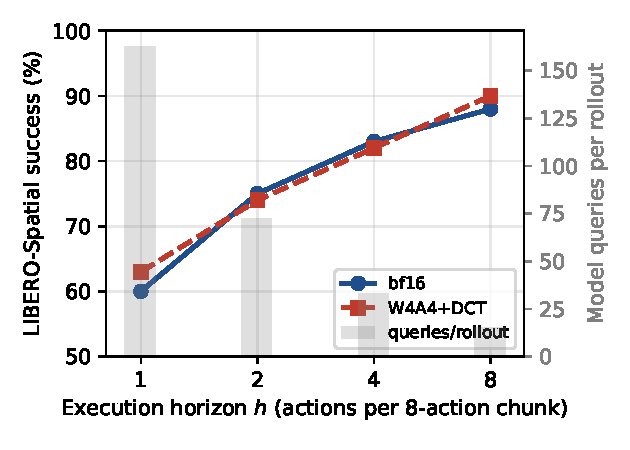
\includegraphics[width=\columnwidth]{horizon_curves}
\caption{Success vs.\ execution horizon $h$ at both precisions (lines, left axis) and
model queries per rollout (bars, right axis). The curves fall in lockstep: the horizon
collapse is precision-independent, and $h{=}8$ is simultaneously the accuracy and the
compute optimum.}
\label{fig:horizon}
\end{figure}

\begin{table}[h]\centering\small
\caption{Execution horizon $h$ vs.\ precision (LIBERO-Spatial, 100 rollouts/cell,
$\pm4\%$ CI).}
\label{tab:horizon}
\begin{tabular}{lcccc}
\toprule
 & $h{=}8$ & $h{=}4$ & $h{=}2$ & $h{=}1$ \\
\midrule
bf16      & 88\% & 83\% & 75\% & 60\% \\
W4A4+DCT  & 90\% & 82\% & 74\% & 63\% \\
\midrule
Queries/rollout & 15.5 & 33.2 & 72.3 & 162.7 \\
Env.\ steps/rollout & 130 & 141 & 154 & 173 \\
\bottomrule
\end{tabular}
\end{table}

Three conclusions. \textbf{(1) The horizon collapse dominates}: 28 points (bf16) from
$h{=}8$ to $h{=}1$---$7\times$ the CI. The mechanism is a train/inference distribution
mismatch: the policy learns to predict chunks from chunk-boundary states; re-querying
mid-motion feeds it out-of-distribution states (arm mid-swing, gripper mid-close) and
induces re-planning dither, corroborated by the 32\% longer trajectories at $h{=}1$.
\textbf{(2) No precision$\times$horizon interaction}: the two curves differ by at most 3
points at any horizon. Fresh feedback does \emph{not} preferentially rescue quantization
error---the hypothesis that quantized policies need tighter closed-loop control is
falsified. \textbf{(3) No tradeoff exists}: $h{=}8$ is simultaneously the accuracy optimum
and the compute optimum (10.5$\times$ fewer queries; at the Jetson Orin's 330\,ms/query,
$h{=}1$ would additionally drop the control rate below 3\,Hz). The deployment rule is one
line: \emph{quantize W4A4+DCT and always execute full chunks.}

% ============================================================================
\section{On-Device Confirmation: Jetson AGX Orin}
\label{sec:device}
% ============================================================================

We deploy the W4A4+DCT quantization stack on a Jetson AGX Orin (NVIDIA, $\sim$\$2k,
60\,W-class)---representative of the vehicle-class compute a mobile robot carries in a
GPS-denied environment. This is \textbf{real packed-INT4 kernel inference}, not simulated
quantization.

\begin{table}[t]\centering\small
\caption{The quantized deployment on real Jetson AGX Orin hardware vs.\ its A100 bf16
reference, both at the official LIBERO-Spatial step budget (220 steps, $10\times10$
rollouts). The $-2.2$\,pt gap is within the $\pm4\%$ binomial CI at 100 rollouts. Power
measured with \texttt{tegrastats} during closed-loop rollouts.}
\label{tab:orin}
\begin{tabular}{lcc}
\toprule
Metric & A100 bf16 & Orin W4A4+DCT \\
\midrule
Closed-loop success & 88.2\% & \textbf{86.0\%} \\
Retention & 100\% & \textbf{97.5\%} \\
Query latency (8-action chunk) & 53\,ms & 330\,ms \\
Effective control rate & $>$100\,Hz & $\approx$24\,Hz \\
Peak memory & 15.4\,GB & $\sim$4.1\,GB (73\%$\downarrow$) \\
Board power (tegrastats) & 300\,W-class & \textbf{20--23.5\,W} \\
Energy per action chunk & --- & \textbf{6.6--7.8\,J} \\
\bottomrule
\end{tabular}
\end{table}

The $-2.2$\,pt gap (86.0\% vs.\ 88.2\%) is within the $\pm4\%$ binomial CI at 100 rollouts:
statistically indistinguishable from the A100 reference. The 330\,ms query yields an
effective control rate of $8/0.33 \approx 24$\,Hz---within the regime required for LIBERO
manipulation. Board power during closed-loop rollouts is 20--23.5\,W (tegrastats),
i.e.\ \textbf{6.6--7.8\,J per 8-action chunk}---an order of magnitude below the
server-GPU power envelope, compatible with battery-powered operation.

To our knowledge this is the \textbf{first real-hardware, closed-loop confirmation of a
quantized L1-regression VLA policy} on edge compute, with power measured in the loop. The
4.1\,GB footprint opens hardware classes previously inaccessible to 7B-parameter VLAs.

% ============================================================================
\section{Comparison to Prior Work}
\label{sec:comparison}
% ============================================================================

\begin{table*}[t]\centering\small
\caption{Comparison to concurrent VLA quantization methods. ``Retention'' = quantized/FP16
success. $\dagger$ Protocol differs: QVLA FP16 baseline 97.1\% vs.\ our 95.5\%.
$\ddagger$ DyQ-VLA targets OpenVLA (token prediction), not OFT (L1-regression).}
\label{tab:comparison}
\begin{tabular}{p{1.9cm}p{2.3cm}p{1.6cm}ccp{2.2cm}p{2.0cm}}
\toprule
Method & Target & Architecture & Precision & Retention & Speedup / Power & Closed-loop Eval \\
\midrule
QuaRot~\cite{quarot} & LLaMA-2-70B & LLM only & W4A4 & $\leq$0.47\,ppl & $3.33\times$ & Perplexity only \\
SpinQuant~\cite{spinquant} & LLaMA-2/3 & LLM only & W4A4 & near-FP & --- & Zero-shot only \\
\midrule
QVLA$^\dagger$~\cite{qvla} & OpenVLA-OFT & L1-reg & W4A4 & 98.9\% & $1.49\times$ & LIBERO + real arm \\
QuantVLA~\cite{quantvla} & $\pi_0$, GR00T & Diffusion & W4A8 & 100.3\% & --- & LIBERO sim only \\
$\Omega$-QVLA~\cite{omegaqvla} & $\pi_{0.5}$, GR00T & Diffusion & W4A4 & $\sim$98--101\% & --- & LIBERO + real \\
DyQ-VLA$^\ddagger$~\cite{dyqvla} & OpenVLA & Token pred. & W4A$\{2,4,8\}$ & 99.5\% & $1.43\times$ & LIBERO + real \\
\midrule
\textbf{Ours} & OpenVLA-OFT & \textbf{L1-reg} & W4A4+DCT & \textbf{99.5\%} sim / \textbf{97.5\%} real & \textbf{20--23.5\,W}, 7\,J/chunk & \textbf{LIBERO + Jetson} \\
\bottomrule
\end{tabular}
\end{table*}

Table~\ref{tab:comparison} positions our work in the concurrent landscape.

\textbf{Vs.\ QVLA.} The closest comparison (same architecture family: OpenVLA-OFT with
L1-regression head). Their 98.9\% retention at W4A4 with a 1.49$\times$ real speedup is
strong; our 99.5\% retention is measured at 400 rollouts against a 95.5\% baseline. Our
distinct contributions: the 16-transform taxonomy, the horizon$\times$precision
interaction study, and closed-loop success \emph{with measured power} on Jetson-class
edge hardware.

\textbf{Vs.\ $\Omega$-QVLA and QuantVLA.} They target diffusion VLAs ($\pi_0$, GR00T),
where per-step DiT activation scaling is a key ingredient not applicable to L1-regression
heads. They report high retention on their targets but no edge-hardware results.

\textbf{Vs.\ DyQ-VLA.} The best concurrent retention (99.5\%) and a measured real-world
speedup (1.43$\times$), on OpenVLA token prediction. Our unique contribution: real-hardware
\emph{task success} and in-the-loop power measurement on edge compute, plus the horizon
study showing dynamic re-querying strategies cannot help at any precision.

% ============================================================================
\section{Discussion and Limitations}
\label{sec:discussion}
% ============================================================================

\textbf{Simulated vs.\ real quantization.} The sweep numbers use fake-quant; the Orin
result is real packed-INT4. The Orin deployment retains 97.5\% of its A100 reference,
indicating no additional real-kernel degradation, but a comprehensive real-kernel sweep
across configurations would strengthen this.

\textbf{Single seed.} All closed-loop numbers are single-seed at their stated rollout
counts; the binomial CIs ($\pm2.5\%$ at 400, $\pm4\%$ at 100) are the resolution limit of
every claim. Differences within CI are reported as parity, never as improvement.

\textbf{One architecture, one benchmark.} Our evidence covers the L1-regression OFT head
on LIBERO. Generalization to diffusion-head VLAs, other benchmarks, and physical-robot
tasks is open.

\textbf{Long-horizon degradation.} The $-$5\,pt W4A4 cost in \textsc{Long} is the main
remaining accuracy target. Task-matched calibration data from the long-horizon suite may
partially recover it.

\textbf{Offline deployment context.} This work targets GPS-denied and
communication-contested environments (AFRL offline autonomy program). The 4.1\,GB
footprint, 24\,Hz control rate, and 20--23.5\,W power draw of the quantized policy are
compatible with battery-powered Jetson-class vehicles for ground and air autonomy.

% ============================================================================
\section{Conclusion}
\label{sec:conclusion}
% ============================================================================

We presented an end-to-end study of VLA policy compression: fine-tuning OpenVLA-OFT on
LIBERO to \textbf{95.5\%} (near-SOTA per suite), a systematic post-training quantization
study, and real edge-hardware deployment. The central message: for L1-regression VLA
control, \emph{activations are the quantization wall}---a single massive-activation
channel makes naive 4-bit activation quantization collapse---and a single orthogonal
rotation is the key: \textbf{W4A4+DCT reaches 95.0\% (99.5\% retention), statistically
indistinguishable from bf16}, while W3A8 trades 5 points for marginal additional
compression. Among 16 candidate transforms, one principle governs all outcomes: global
dense mixers spread energy and work; PCA concentrates energy and is harmful. The
execution-horizon study adds an orthogonal deployment rule: truncating action chunks
collapses success identically at every precision---chunked execution is load-bearing,
quantization is free, and full-chunk W4A4+DCT is simultaneously the accuracy and the
compute optimum. Real Jetson AGX Orin deployment confirms the result where it matters:
97.5\% retention at a 24\,Hz control rate, in 4.1\,GB and 20--23.5\,W.

% ============================================================================

\begin{thebibliography}{99}
\small

\bibitem{openvla}
  M.~J.~Kim et al., ``OpenVLA: An Open-Source Vision-Language-Action Model,''
  in \textit{CoRL}, 2024. arXiv:2406.09246.

\bibitem{openvlaoft}
  M.~J.~Kim, C.~Finn, and P.~Liang, ``Fine-Tuning Vision-Language-Action Models:
  Optimizing Speed and Success,'' \textit{arXiv:2502.19645}, 2025.

\bibitem{libero}
  B.~Liu et al., ``LIBERO: Benchmarking Knowledge Transfer for Lifelong Robot Learning,''
  in \textit{NeurIPS}, 2023.

\bibitem{gptq}
  E.~Frantar et al., ``GPTQ: Accurate Post-Training Quantization for Generative
  Pre-trained Transformers,'' in \textit{ICLR}, 2023.

\bibitem{awq}
  J.~Lin et al., ``AWQ: Activation-aware Weight Quantization for LLM Compression and
  Acceleration,'' in \textit{MLSys}, 2024.

\bibitem{smoothquant}
  G.~Xiao et al., ``SmoothQuant: Accurate and Efficient Post-Training Quantization for
  Large Language Models,'' in \textit{ICML}, 2023.

\bibitem{quarot}
  S.~Ashkboos et al., ``QuaRot: Outlier-Free 4-Bit Inference in Rotated LLMs,''
  in \textit{NeurIPS}, 2024. arXiv:2404.00456.

\bibitem{spinquant}
  Z.~Liu et al., ``SpinQuant: LLM Quantization with Learned Rotations,''
  in \textit{ICLR}, 2025.

\bibitem{quip}
  A.~Tseng et al., ``QuIP\#: Even Better LLM Quantization with Hadamard Incoherence and
  Lattice Codebooks,'' in \textit{ICML}, 2024.

\bibitem{sun2024massive}
  M.~Sun et al., ``Massive Activations in Large Language Models,''
  \textit{arXiv:2402.17762}, 2024.

\bibitem{qvla}
  Y.~Xu et al., ``QVLA: Not All Channels Are Equal in Vision-Language-Action Model's
  Quantization,'' \textit{arXiv:2602.03782}, 2026.

\bibitem{quantvla}
  J.~Zhang et al., ``QuantVLA: Scale-Calibrated Post-Training Quantization for
  Vision-Language-Action Models,'' \textit{arXiv:2602.20309}, 2026.

\bibitem{omegaqvla}
  X.~Wang et al., ``$\Omega$-QVLA: Robust Quantization for Vision-Language-Action Models
  via Composite Rotation and Per-step Scaling,'' \textit{arXiv:2605.28803}, 2026.

\bibitem{dyqvla}
  Z.~Zheng et al., ``DyQ-VLA: Temporal-Dynamic-Aware Quantization for Embodied
  Vision-Language-Action Models,'' \textit{arXiv:2603.07904}, 2026.

\end{thebibliography}

\end{document}
